\documentclass{article}
\usepackage{tikz}
\usetikzlibrary{snakes}
\usetikzlibrary{positioning}
\usetikzlibrary{calc}
\tikzset{
  pics/carc/.style args={#1:#2:#3}{
    code={
      \draw[pic actions] (#1:#3) arc(#1:#2:#3);
    }
  }
}
\begin{document}
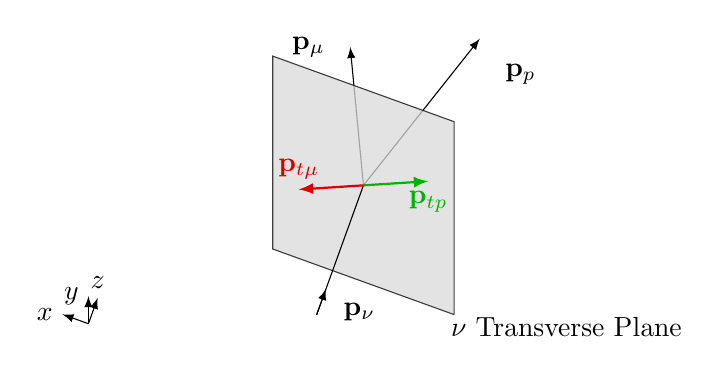
\begin{tikzpicture}[x={(-0.94cm,0.34cm)}, y={(0cm,1cm)}, z={(0.34cm,0.94cm)}, scale=0.35]

% coordinate system
\coordinate (O) at (7, 2, -5);
\draw[-latex] (O) -- +(1, 0,  0) node [left] {$x$};
\draw[-latex] (O) -- +(0,  1, 0) node [left] {$y$};
\draw[-latex] (O) -- +(0,  0, 1) node [above] {$z$};

\coordinate (NDP) at (0,0,0);
\coordinate (VERT) at (0,0,5);

%NDXYPlane1
% \draw[fill=black!30!white] ($ (VERT) - (0,3,0) $) -- ($ (VERT) - (2.997,3,0.13) $) -- ($ (VERT) - (2.997,-3,0.13) $) -- ($ (VERT) + (0,3,0) $);

%%%Outgoing full
\draw[-latex] (VERT) -- ($ (VERT) + (2.5,-1,5.5) $) node [left = .2cm] {$\mathbf{p}_\mu$};
\draw[-latex] (VERT) -- ($ (VERT) + (-2.5,1,5.5) $) node [below right = 0.2cm and 0.2cm] {$\mathbf{p}_p$};

% \draw[fill=black!15!white,opacity=0.75] ($ (VERT) - (3,3,0) $) -- ($ (VERT) - (3,-3,0) $) -- ($ (VERT) + (3,3,0) $) -- ($ (VERT) + (3,-3,0) $) -- ($ (VERT) - (3,3,0) $);

\draw[fill=black!15!white,opacity=0.75] ($ (VERT) - (3.5,3.5,0) $) -- ($ (VERT) - (3.5,-3.5,0) $) -- ($ (VERT) + (3.5,3.5,0) $) -- ($ (VERT) + (3.5,-3.5,0) $) -- ($ (VERT) - (3.5,3.5,0) $);

%NDXYPlane2
% \draw[fill=black!30!white] ($ (VERT) + (0,3,0) $) -- ($ (VERT) + (2.997,3,0.13) $) -- ($ (VERT) + (2.997,-3,0.13) $) -- ($ (VERT) - (0,3,0) $);

% \draw ($ (VERT) + (3,3,0) $) node [above] {ND280 X-Y Plane};
\draw ($ (VERT) - (3,2,0) $) node [below right = 0.5cm and 0.001cm] {$\nu$ Transverse Plane};

\draw (NDP) -- (VERT);
\draw[-latex] (NDP) -- ($ (NDP) + (0,0,1) $) node [below right = 0.05cm and 0.1cm] {$\mathbf{p}_\nu$};

%%%Outgoing transverse
\draw[-latex,black!15!red, thick] (VERT) -- ($ (VERT) + (2.5,-1,0) $) node [above] {$\mathbf{p}_{t\mu}$};
\draw[-latex,black!30!green, thick] (VERT) -- ($ (VERT) + (-2.5,1,0) $) node [below] {$\mathbf{p}_{tp}$};


\end{tikzpicture}

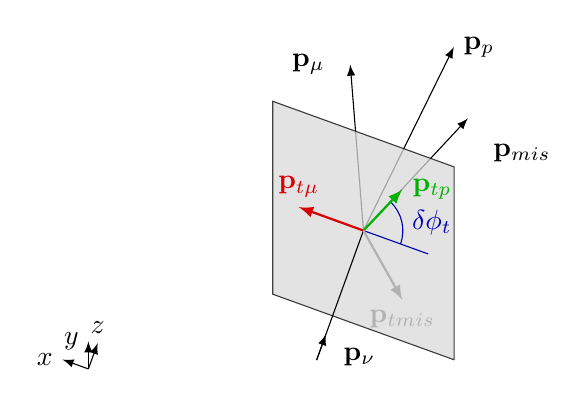
\begin{tikzpicture}[x={(-0.94cm,0.34cm)}, y={(0cm,1cm)}, z={(0.34cm,0.94cm)}, scale=0.35]

% coordinate system
\coordinate (O) at (7, 2, -5);
\draw[-latex] (O) -- +(1, 0,  0) node [left] {$x$};
\draw[-latex] (O) -- +(0,  1, 0) node [left] {$y$};
\draw[-latex] (O) -- +(0,  0, 1) node [above] {$z$};

\coordinate (NDP) at (0,0,0);
\coordinate (VERT) at (0,0,5);

%NDXYPlane1
% \draw[fill=black!30!white] ($ (VERT) - (0,3,0) $) -- ($ (VERT) - (2.997,3,0.13) $) -- ($ (VERT) - (2.997,-3,0.13) $) -- ($ (VERT) + (0,3,0) $);

%%%Outgoing full
\draw[-latex] (VERT) -- ($ (VERT) + (2.5,0,5.5) $) node [left = .2cm] {$\mathbf{p}_\mu$};
\draw[-latex] (VERT) -- ($ (VERT) + (-1.5,2,5.5) $) node [right] {$\mathbf{p}_p$};
\draw[-latex] (VERT) -- ($ (VERT) + (-1.5,-2,7.0) $) node [below right = 0.2cm and 0.2cm] {$\mathbf{p}_{mis}$};

% \draw[fill=black!15!white,opacity=0.75] ($ (VERT) - (3,3,0) $) -- ($ (VERT) - (3,-3,0) $) -- ($ (VERT) + (3,3,0) $) -- ($ (VERT) + (3,-3,0) $) -- ($ (VERT) - (3,3,0) $);

\draw[fill=black!15!white,opacity=0.75] ($ (VERT) - (3.5,3.5,0) $) -- ($ (VERT) - (3.5,-3.5,0) $) -- ($ (VERT) + (3.5,3.5,0) $) -- ($ (VERT) + (3.5,-3.5,0) $) -- ($ (VERT) - (3.5,3.5,0) $);

%NDXYPlane2
% \draw[fill=black!30!white] ($ (VERT) + (0,3,0) $) -- ($ (VERT) + (2.997,3,0.13) $) -- ($ (VERT) + (2.997,-3,0.13) $) -- ($ (VERT) - (0,3,0) $);

% \draw ($ (VERT) + (3,3,0) $) node [above] {ND280 X-Y Plane};
% \draw ($ (VERT) - (3,2,0) $) node [below right = 0.5cm and 0.001cm] {$\nu$ Transverse Plane};

\draw (NDP) -- (VERT);
\draw[-latex] (NDP) -- ($ (NDP) + (0,0,1) $) node [below right = 0.05cm and 0.1cm] {$\mathbf{p}_\nu$};

\draw[black!30!blue] (VERT) -- ($ (VERT) - (2.5,0,0) $);
\draw[black!30!blue] (VERT) pic{carc = -20:47:0.5cm};
\draw[black!30!blue] ($ (VERT) - (1.5,-0.8,0) $) node [right] {$\delta\phi_t$};

%%%Outgoing transverse
\draw[-latex,black!15!red, thick] (VERT) -- ($ (VERT) + (2.5,0,0) $) node [above] {$\mathbf{p}_{t\mu}$};
\draw[-latex,black!30!green, thick] (VERT) -- ($ (VERT) + (-1.5,2,0) $) node [right] {$\mathbf{p}_{tp}$};
\draw[-latex,black!30!white, thick] (VERT) -- ($ (VERT) + (-1.5,-2,0) $) node [below] {$\mathbf{p}_{tmis}$};


\end{tikzpicture}

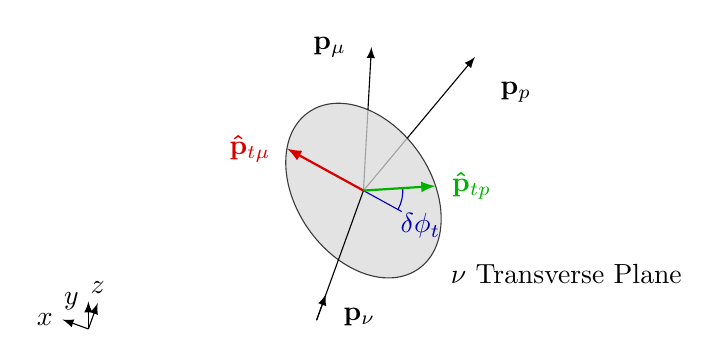
\begin{tikzpicture}[x={(-0.94cm,0.34cm)}, y={(0cm,1cm)}, z={(0.34cm,0.94cm)}, scale=0.35]

% coordinate system
\coordinate (O) at (7, 2, -5);
\draw[-latex] (O) -- +(1, 0,  0) node [left] {$x$};
\draw[-latex] (O) -- +(0,  1, 0) node [left] {$y$};
\draw[-latex] (O) -- +(0,  0, 1) node [above] {$z$};

\coordinate (NDP) at (0,0,0);
\coordinate (VERT) at (0,0,5);

%NDXYPlane1
% \draw[fill=black!30!white] ($ (VERT) - (0,3,0) $) -- ($ (VERT) - (2.997,3,0.13) $) -- ($ (VERT) - (2.997,-3,0.13) $) -- ($ (VERT) + (0,3,0) $);

%%%Outgoing full
\draw[-latex] (VERT) -- ($ (VERT) + (1.5,0,5) $) node [left = .2cm] {$\mathbf{p}_\mu$};
\draw[-latex] (VERT) -- ($ (VERT) + (-2.5,1,5) $) node [below right = 0.2cm and 0.2cm] {$\mathbf{p}_p$};

% \draw[fill=black!15!white,opacity=0.75] ($ (VERT) - (3,3,0) $) -- ($ (VERT) - (3,-3,0) $) -- ($ (VERT) + (3,3,0) $) -- ($ (VERT) + (3,-3,0) $) -- ($ (VERT) - (3,3,0) $);

\draw[fill=black!15!white,opacity=0.75] (VERT) circle (3);
%NDXYPlane2
% \draw[fill=black!30!white] ($ (VERT) + (0,3,0) $) -- ($ (VERT) + (2.997,3,0.13) $) -- ($ (VERT) + (2.997,-3,0.13) $) -- ($ (VERT) - (0,3,0) $);

% \draw ($ (VERT) + (3,3,0) $) node [above] {ND280 X-Y Plane};
\draw ($ (VERT) - (3,2,0) $) node [right] {$\nu$ Transverse Plane};

\draw (NDP) -- (VERT);
\draw[-latex] (NDP) -- ($ (NDP) + (0,0,1) $) node [below right = 0.05cm and 0.1cm] {$\mathbf{p}_\nu$};
%ref +x line
\draw[black!30!blue] (VERT) -- ($ (VERT) - (1.48,0.260,0) $);
\draw[black!30!blue] (VERT) pic{carc = -29:5:0.5cm};
\draw[black!30!blue] ($ (VERT) - (1,0,0) $) node [below right = 0.05cm and 0.02cm] {$\delta\phi_t$};

%%%Outgoing transverse
\draw[-latex,black!15!red, thick] (VERT) -- ($ (VERT) + (2.95,0.521,0) $) node [left = 0.08cm] {$\mathbf{\hat{p}}_{t\mu}$};
\draw[-latex,black!30!green, thick] (VERT) -- ($ (VERT) + (-2.784,1.113,0) $) node [right = 0.08cm] {$\mathbf{\hat{p}}_{tp}$};


\end{tikzpicture}

\end{document}
